


\section{Intergranular Stress Corrosion Cracking}

Stress corrosion cracking may be trans granular (through the grains) or intergranular, at the grain boundary.  IGSCC is a particularly prominent failure mechnism for Austenitic stainless steels.  For IGSCC to occur, there must be a material that is susceptible to this form of cracking, an environment that is corrosive to the material as well as stress.  

Stress may come from a high pressure environment, residual stress due to welding.  In a reactor, the atomic structure may be under stress due to damage caused by neutrons passing through the steel, or due to the swelling of the steel on the macroscopic scale.  If chromium is depleted at the grain boundary, protection to corrosion due to the passive layer is lost.  This, coupled with the knowledge that austenitic stainless steels are susceptible to IGSCC, completes the three requirements and, over time, components of this material in these conditions will eventually fail to IGSCC.

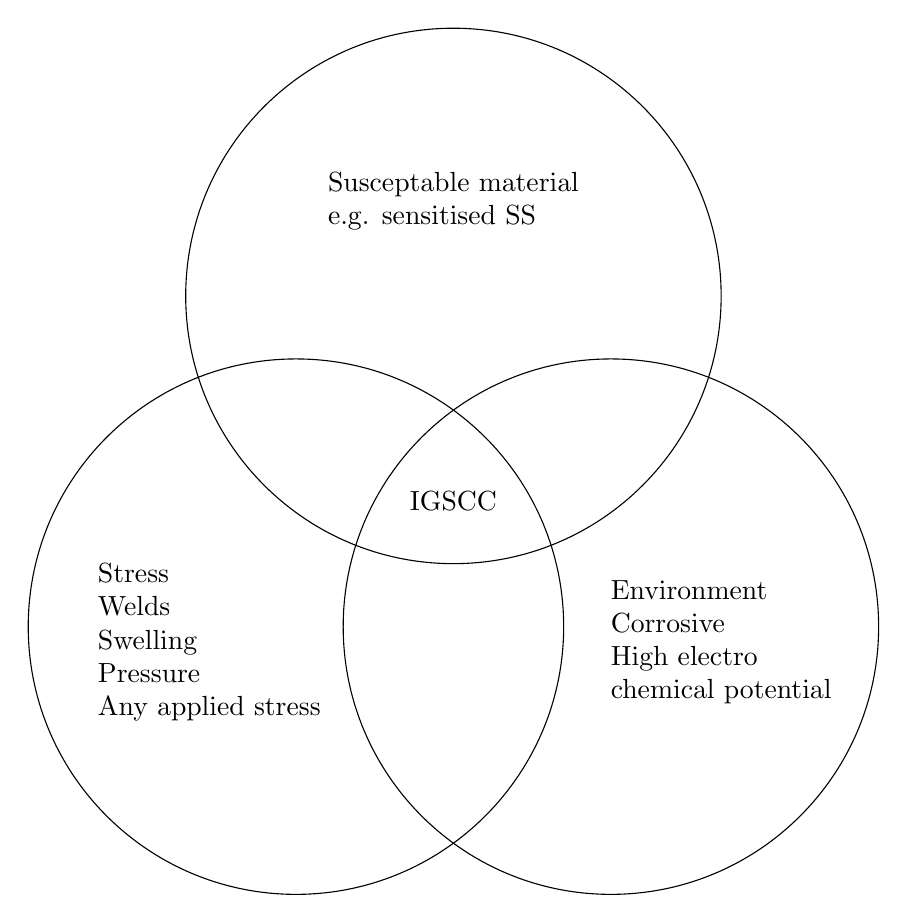
\begin{tikzpicture}
\draw (4.5,5.0) circle [radius=3.4];
\draw (2.5,0.8) circle [radius=3.4];
\draw (6.5,0.8) circle [radius=3.4];
\node[align=left] at (4.5, 2.4) {IGSCC};
\node[align=left] at (1.4,0.6) {Stress\\Welds\\Swelling\\Pressure\\Any applied stress};
\node[align=left] at (4.5, 6.2) {Susceptable material \\ e.g. sensitised SS};
\node[align=left] at (7.9,0.6) {Environment\\ Corrosive\\ High electro \\chemical potential};
\end{tikzpicture}

IGSCC has not only been a defect in stainless steel.  High Nickel content alloys, such as Alloy 600 (Inconel:  Ni-72, Cr-17, Fe-10),  have been known to suffer from IGSCC since the very early days of nuclear energy, in particular with the prototype S1W reactor, prototype for the first nuclear powered submarine, the USS Nautilus.

Austenitic stainless steels, primarily stabilised in the FCC structure due to the addition of Nickel, also suffer from IGSCC.  

\begin{figure}[tbp]
  \begin{center}
    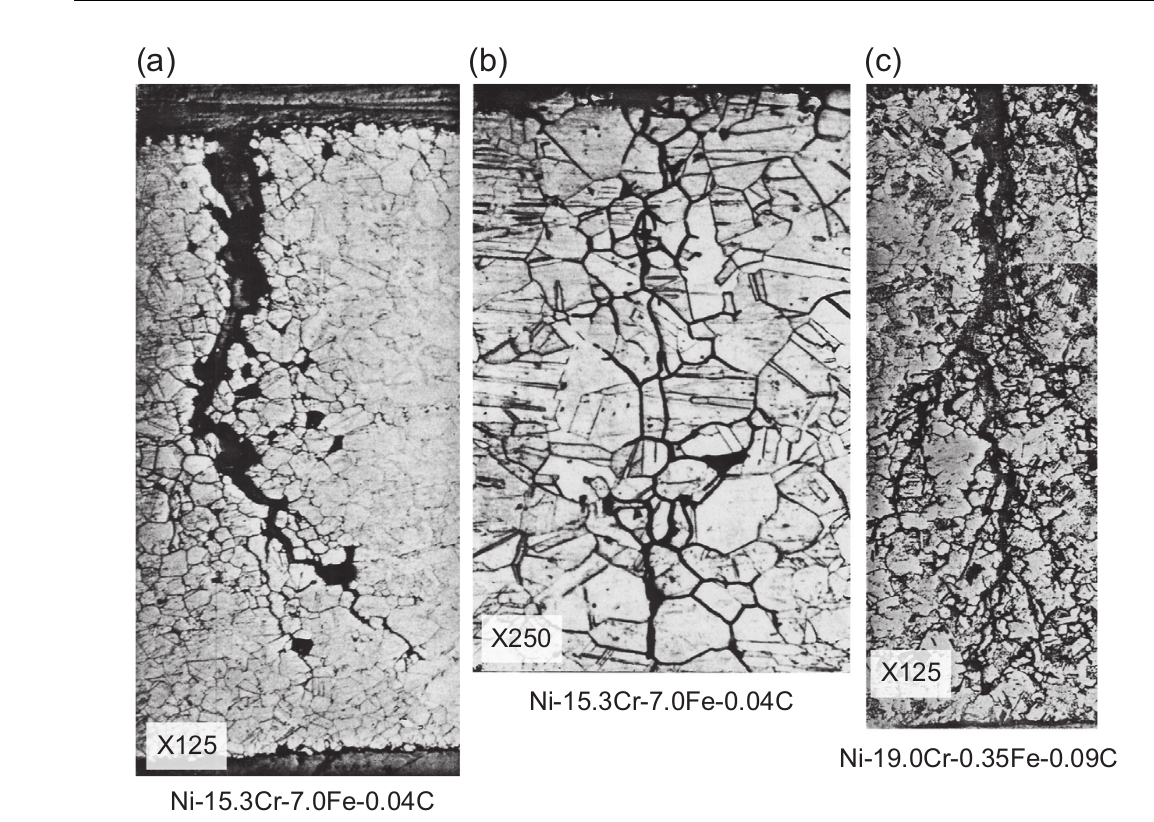
\includegraphics[width=7.0cm]{chapters/background_austenitic_steels_in_nuclear/images/igscc_nickel_alloy600.png}
    \caption{Graph caption}
    \label{image:flux1}
  \end{center}
\end{figure}








\subsection{Sensitisation and IGSCC}









\subsection{IGSCC in Advanced Gas-cooled Reactors}

The first generation of nuclear reactors in the UK were Magnox type reactors.  They used unenriched Uranium 0.7% U235 as fuel which was contained within magnesium oxide cladding due to its low absorption cross section.  A major drawback was the relatively low operating temperature of 360C.

Carnot's theorem shows that the maximum amount of energy from an engine is dependent on the difference between the hot and cold reservoirs.  The ambient temperature of the powerstation will vary a small amount with the seasons.  The practical way to improve the maximum possible efficiency is to increase the engine (reactor) temperature.

\begin{equation}
\begin{split}
\eta_{max} = 1 - \frac{T_c}{T_h}
\text{where the temperature is measured in absoute units}
\end{split}
\end{equation}

AGRs were designed to run at much higher temperatures of 650C.  By increasing the temperature, the maximum possible thermal efficiency was increased from just over 50 percent to almost 70 percent.  To withstand higher temperatures, the fuel cladding needed to be changed.  Steel cladding was contained 2.3% U235 Uranium, enriched to counter the higher absorpbtion cross section of the new material.

The $CO_{2}$ 





\subsection{IGSCC in Advanced Gas-cooled Reactors}




 

